% !Mode:: "TeX:UTF-8"
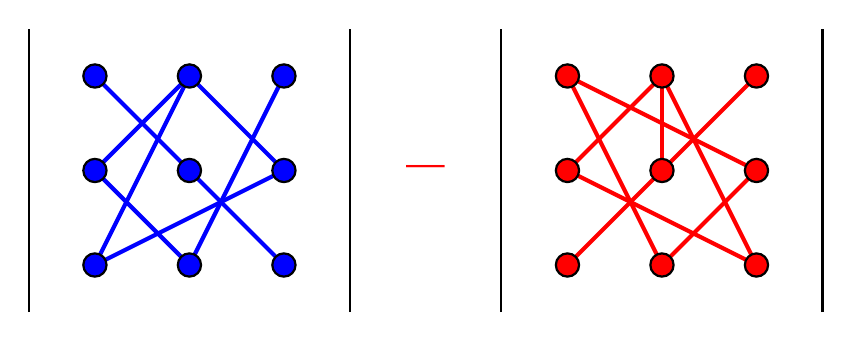
\begin{tikzpicture}[scale=1.2, line width=1.5pt]

  % === LEFT PART (POSITIVE TERMS, BLUE) ===
  \draw[thick] (-0.7, -0.5) -- (-0.7, 2.5);
  \draw[thick] (2.7, -0.5) -- (2.7, 2.5);

  \foreach \x in {0, 1, 2} {
    \foreach \y in {0, 1, 2} {
      \coordinate (L-\x-\y) at (\x, \y);
    }
  }

  \draw[blue] (L-0-2) -- (L-1-1) -- (L-2-0);
  \draw[blue] (L-0-1) -- (L-1-2) -- (L-2-1);
  \draw[blue] (L-0-0) -- (L-2-1);
  \draw[blue] (L-0-1) -- (L-1-0);
  \draw[blue] (L-1-0) -- (L-2-2);
  \draw[blue] (L-0-0) -- (L-1-2);

  \foreach \x in {0, 1, 2} {
    \foreach \y in {0, 1, 2} {
      \filldraw[fill=blue, draw=black, thick] (L-\x-\y) circle (3.5pt);
    }
  }

  % === MINUS SIGN IN THE MIDDLE ===
  \node at (3.5, 1) {\Huge\bfseries\color{red} --};

  % === RIGHT PART (NEGATIVE TERMS, RED) ===
  \draw[thick] (4.3, -0.5) -- (4.3, 2.5);
  \draw[thick] (7.7, -0.5) -- (7.7, 2.5);

  \foreach \x in {5, 6, 7} {
    \foreach \y in {0, 1, 2} {
      \coordinate (R-\x-\y) at (\x, \y);
    }
  }

  \draw[red] (R-5-2) -- (R-7-1);
  \draw[red] (R-5-1) -- (R-6-2) -- (R-7-0);
  \draw[red] (R-5-0) -- (R-7-2);
  \draw[red] (R-5-2) -- (R-6-0);
  \draw[red] (R-6-0) -- (R-7-1);
  \draw[red] (R-5-1) -- (R-7-0);
  \draw[red] (R-6-2) -- (R-6-1);

  \foreach \x in {5, 6, 7} {
    \foreach \y in {0, 1, 2} {
      \filldraw[fill=red, draw=black, thick] (R-\x-\y) circle (3.5pt);
    }
  }

\end{tikzpicture}